\documentclass[12pt, a4paper]{article}
\usepackage{esvect}
\usepackage{amsmath}
\usepackage{eso-pic}
\usepackage{pdfpages}
\usepackage{graphicx}
\usepackage[utf8]{inputenc}
\usepackage[svgnames]{xcolor}
\usepackage{tcolorbox}
\usepackage{listings}
\usepackage{hyperref}
\usepackage{titling}
\usepackage{listings}
\lstset{breaklines=true,}
\usepackage[T1]{fontenc}
\newtheorem{def}{Definição}
\newtheorem{reso}{Resolução}
%\renewcommand*\familydefault{\sfdefault}

\title{Cálculo de PCA}
\author{Ronaldo Pacheco Pereira
\and Andressa dos Santos Silva}
\begin{document}
\maketitle

\section{PCA - Principal Component Analysis}


\textbf{Os principais objetivos do PCA são:}\\
\begin{itemize}
\item Redução de dimensionalidade: O PCA permite reduzir a dimensionalidade de um conjunto de dados, mantendo a maior parte da variabilidade dos dados. Isso é especialmente útil quando se lida com conjuntos de dados com muitas variáveis, tornando-os mais fáceis de visualizar, analisar e interpretar.

\item Eliminação de correlações: Os componentes principais são não correlacionados entre si. Isso pode ser vantajoso quando se lida com variáveis altamente correlacionadas, pois simplifica a interpretação dos resultados e evita problemas de multicolinearidade em análises posteriores.

\item Identificação de padrões: O PCA pode revelar padrões e estruturas latentes nos dados, destacando as variáveis que mais contribuem para a variação dos dados. Isso pode ajudar a identificar grupos, clusters ou tendências nos dados.
\end{itemize}
Além disso, o PCA também pode ser usado para visualizar os dados em um espaço de menor dimensionalidade, permitindo a criação de gráficos de dispersão ou projeções em 2D ou 3D que facilitam a interpretação e a detecção de padrões.

No entanto, é importante notar que o PCA é sensível à escala dos dados e pressupõe que os dados sejam linearmente correlacionados. Portanto, é comum normalizar os dados antes de aplicar o PCA para garantir que todas as variáveis tenham a mesma importância.

\subsection{Cálculo de PCA}

Suponha que você tenha um conjunto de dados representado por uma matriz $X$, onde cada linha representa uma observação e cada coluna representa uma variável. A matriz $X$ tem dimensões $m \times n$, onde $m$ é o número de observações e $n$ é o número de variáveis.

\begin{enumerate}
  \item Calcule a matriz de covariância $C$ dos dados de entrada $X$:

  \[
  C = \frac{(X - \mu)(X - \mu)^T}{(m - 1)}
  \]

  onde $\mu$ é o vetor médio das colunas de $X$ e $(X - \mu)^T$ é a transposição da matriz $(X - \mu)$.

  \item Realize a decomposição de valores singulares (SVD) na matriz de covariância $C$:

  \[
  C = U \Sigma V^T
  \]

  onde $U$ é uma matriz ortogonal $m \times m$ que contém os vetores próprios (componentes principais) do conjunto de dados, $\Sigma$ é uma matriz diagonal $m \times n$ que contém os valores singulares e $V$ é uma matriz ortogonal $n \times n$.

  \item Selecione os $k$ componentes principais mais importantes com base nos valores singulares correspondentes. Geralmente, os componentes principais são ordenados em ordem decrescente com base nos valores singulares.

  \item Projete os dados originais $X$ no espaço dos componentes principais selecionados:

  \[
  Y = XW
  \]

  onde $Y$ é a matriz de dados projetada, $W$ é uma matriz de pesos obtida a partir dos $k$ componentes principais selecionados e é calculada como:

  \[
  W = V(:, :k)
  \]

  onde $V(:, :k)$ representa as primeiras $k$ colunas da matriz $V$.

\subsection{Interpretação do resultado do PCA}
A interpretação do resultado do PCA resumidamente envolve entender as principais componentes, que são as direções de máxima variabilidade nos dados, e os valores singulares, que indicam a importância de cada componente. A análise se concentra em compreender como as componentes contribuem para a variabilidade dos dados e quais são as mais relevantes para explicar as características dos dados.

\subsection{Aplicações em Data Science}

A Análise de Componentes Principais (PCA) é uma técnica estatística amplamente utilizada em Data Science para simplificar conjuntos de dados complexos, reduzindo sua dimensionalidade. O PCA é aplicado em uma variedade de problemas, como análise exploratória de dados, visualização, pré-processamento de dados e extração de características.

O PCA tem várias aplicações em Data Science:

\begin{itemize}
    \item Redução de dimensionalidade: O PCA ajuda a lidar com conjuntos de dados de alta dimensionalidade, onde existem muitas variáveis. Ele identifica as combinações lineares das variáveis originais que capturam a maior parte da variabilidade dos dados. Isso permite representar os dados em um espaço de menor dimensão, mantendo a maior parte das informações relevantes.
    
    \item Detecção de padrões: O PCA pode ser usado para encontrar padrões ocultos em dados. Ao identificar as principais direções de variabilidade nos dados, o PCA revela as relações mais significativas entre as variáveis. Isso pode ajudar a identificar agrupamentos, estruturas ou anomalias nos dados.
    
    \item Visualização de dados: O PCA é frequentemente usado para visualizar conjuntos de dados complexos em espaços bidimensionais ou tridimensionais. Ele projeta os dados em componentes principais selecionados, permitindo uma representação gráfica mais simples e compreensível. Isso pode facilitar a identificação de grupos de dados, tendências ou separação de classes.
    
    \item Pré-processamento de dados: O PCA pode ser usado como uma etapa de pré-processamento para melhorar a eficiência e a precisão de algoritmos de aprendizado de máquina. Ao reduzir a dimensionalidade dos dados, o PCA ajuda a eliminar características redundantes ou ruidosas, melhorando o desempenho dos modelos.
    
    \item Extração de características: O PCA também pode ser usado para extrair características importantes dos dados. Ao selecionar um número menor de componentes principais, o PCA pode fornecer uma representação compacta dos dados originais. Essas características extraídas podem ser usadas como entrada para outros algoritmos de aprendizado de máquina ou como entrada para técnicas de clustering e classificação.
    \end{itemize}

    
Em resumo, o PCA é uma ferramenta poderosa em Data Science que permite a redução da dimensionalidade, identificação de padrões, visualização de dados e pré-processamento eficiente. Ele ajuda os cientistas de dados a lidar com conjuntos de dados complexos, melhorar a eficiência dos modelos e obter insights valiosos a partir dos dados.
\section{PyCharm IDE Python}

Para esse trabalho, foi utilizado a IDE PyCharm (Python).
O PyCharm é um IDE para Python, disponível em duas edições, Community e Professional. O mesmo possui recursos para autocompletar código, depuração, refatoração, testes automatizados e integração com controle de versão. O PyCharm inclui um gerenciador de projetos, terminal integrado e suporte a diferentes interpretes Python e ambientes virtuais. Além disso, oferece suporte a plugins para desenvolvimento em outras linguagens e plataformas. O PyCharm é amplamente utilizado por programadores e equipes de desenvolvimento em todo o mundo.

\section{Bibliotecas utilizadas em Python}
Abaixo a relação de bibliotecas utilizadas nesse trabalho.
\begin{center}
    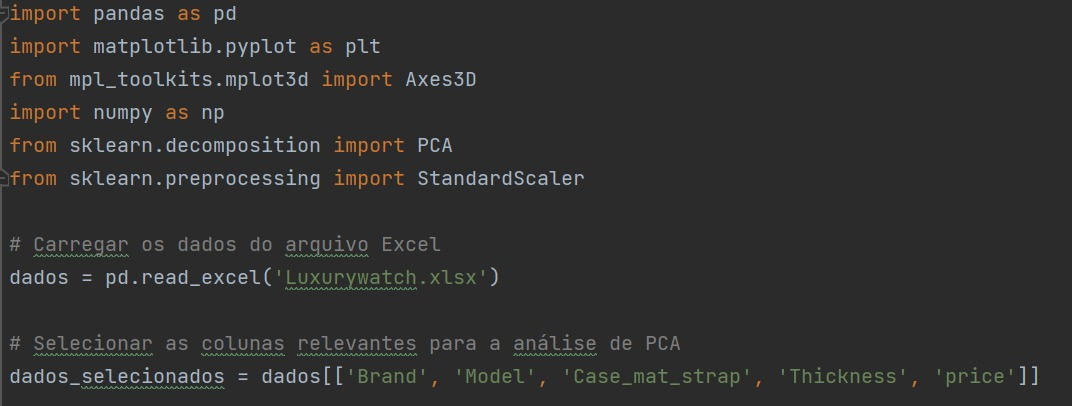
\includegraphics[width=14cm]{figura1}
 \textbf{Biblioteca e carregamento dos dados do arquivo. 
Seleção dos dados relevantes para analise de PCA}   
\end{center}

\textbf{Pandas:}\\
Biblioteca para manipulação e análise de dados em Python, oferecendo estruturas de dados flexíveis e eficientes para lidar com conjuntos de dados tabulares.

\textbf{NumPy:}\\
Uma biblioteca popular de aprendizado de máquina em Python, que inclui a classe PCA para realizar a Análise de Componentes Principais.
\textbf{Scikit-learn:}\\
Uma biblioteca popular de aprendizado de máquina em Python, que inclui a classe PCA para realizar a Análise de Componentes Principais.

\textbf{StandardScaler:}\\
Uma classe do Scikit-learn que realiza a padronização dos dados, transformando-os para ter média zero e desvio padrão unitário, o que é útil para pré-processamento de dados antes de aplicar algoritmos de aprendizado de máquina.

\textbf{MatPlotLib.Pyplot:}\\
Biblioteca para visualização de dados em Python, permitindo a criação de gráficos e plotagens de forma personalizada.\\
\textbf{mpltoolkits.mplot3d:}\\Um módulo do Matplotlib que fornece recursos para criar gráficos em 3D.\\


\subsection{Dados Qualitativos}
Os Dados foram baixados no site Kaggle e após ser limpo de inconsistências e erros, foi importado e agregado usando o pandas no formato final Xlsx, deixando assim, somente a informação util ao trabalho final.


\subsection{Metodologia}

\begin{center}
    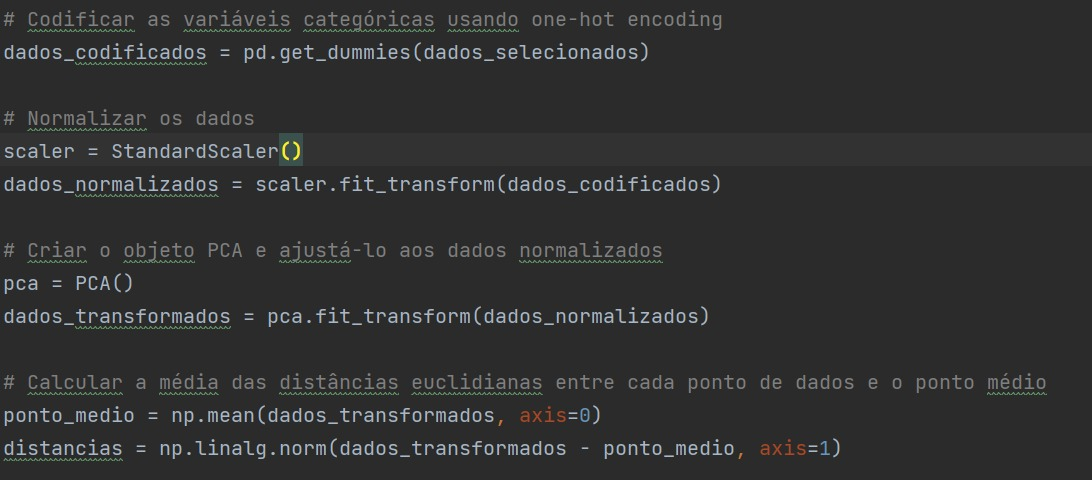
\includegraphics[width=14cm]{figura2}
 \textbf{Normalização dos dados para dar maior acurácia durante a analise de PCA. Calculo de média das distâncias euclidianas para determinar o dado com autovalor mais significativo.}  
\end{center}

\begin{center}
    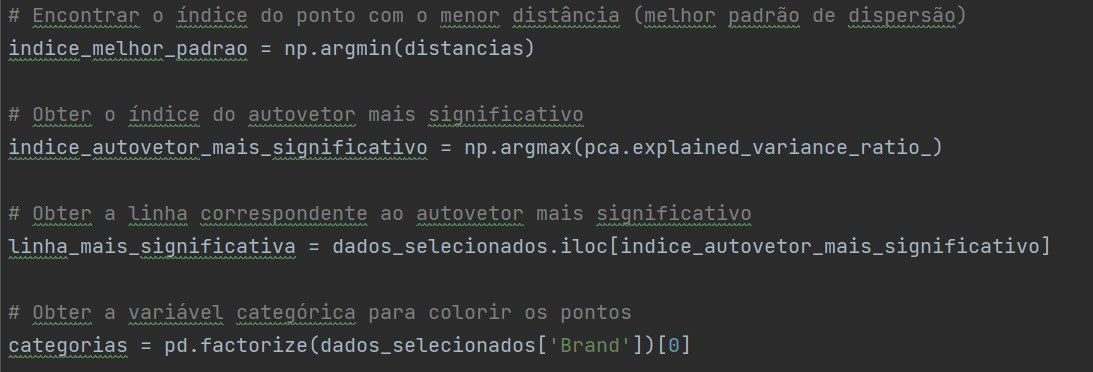
\includegraphics[width=14cm]{figura 3.jpg}
\end{center} 

\textbf{Importação de bibliotecas:}

\begin{verbatim}

import pandas as pd  % Importa a biblioteca Pandas para manipulação e 
análise de dados.

import matplotlib.pyplot as plt  % Importa a biblioteca Matplotlib 
para visualização de gráficos.

from mpl_toolkits.mplot3d import Axes3D  % Importa a classe Axes3D 
da biblioteca mpl_toolkits.mplot3d para criar gráficos em 3D.
import numpy as np  % Importa a biblioteca NumPy para operações 
matemáticas.

from sklearn.decomposition import PCA  % Importa a classe PCA da 
biblioteca scikit-learn para realizar a análise de Componentes Principais.
from sklearn.preprocessing import StandardScaler  % Importa a 
classe StandardScaler da biblioteca scikit-learn para normalizar os dados.
\end{verbatim}

\textbf{Carregar os dados:}

\begin{verbatim}
dados = pd.read_excel('Luxurywatch.xlsx')  % Lê um arquivo Excel 
chamado 'Luxurywatch.xlsx' e armazena os dados em um objeto DataFrame 
chamado 'dados'.
\end{verbatim}

\textbf{Selecionar colunas relevantes:}

\begin{verbatim}
dados_selecionados = dados[['Brand', 'Case_mat_strap', 
'Thickness', 'price']]  % Seleciona as colunas relevantes para a 
análise de PCA, que são 'Brand', 'Case_mat_strap', 
'Thickness' e 'price', e armazena os dados em um novo DataFrame 
chamado 'dados_selecionados'.
\end{verbatim}

\textbf{Codificar variáveis categóricas:}

\begin{verbatim}
dados_codificados = pd.get_dummies(dados_selecionados)  % Codifica 
as variáveis categóricas do DataFrame 'dados_selecionados'
usando o método de codificação one-hot encoding e armazena 
os dados no DataFrame 'dados_codificados'.
\end{verbatim}

\textbf{Normalizar os dados:}

\begin{verbatim}
scaler = StandardScaler()  % Cria um objeto StandardScaler 
para normalizar os dados.
dados_normalizados = scaler.fit_transform(dados_codificados) 
% Normaliza os dados do DataFrame 'dados_codificados' usando 
o objeto StandardScaler criado anteriormente e armazena os 
dados normalizados no DataFrame 'dados_normalizados'.
\end{verbatim}

\textbf{Criar objeto PCA e ajustá-lo aos dados normalizados:}

\begin{verbatim}
pca = PCA()  % Cria um objeto PCA.
dados_transformados = pca.fit_transform(dados_normalizados) 
% Ajusta o objeto PCA aos dados normalizados do DataFrame 
'dados_normalizados' e transforma os dados para um novo 
espaço de características. Os dados transformados são 
armazenados no DataFrame 'dados_transformados'.
\end{verbatim}

\textbf{Imprimir o tamanho da matriz de autovetores:}

\begin{verbatim}
print("Tamanho da Matriz de Autovetores:", pca.components_.shape)  
% Imprime o tamanho da matriz de autovetores, que representa 
os vetores próprios (autovetores) do PCA.
\end{verbatim}

\textbf{Imprimir o autovalor mais significativo:}

\begin{verbatim}
autovalor_mais_significativo = pca.explained_variance_[0]  
% Obtém o autovalor mais significativo, que é o primeiro 
valor do array 'explained_variance_' do objeto PCA.
print("Autovalor Mais Significativo:", 
autovalor_mais_significativo)  % Imprime o autovalor 
mais significativo.
\end{verbatim}

\textbf{Identificar a linha com o autovetor mais significativo:}

\begin{verbatim}
indice_autovetor_mais_significativo = np.argmax
(pca.components_[0])  % Encontra o índice do autovetor 
mais significativo, que é o índice do valor máximo 
do primeiro elemento da matriz 'components_' do objeto PCA.
linha_mais_significativa = dados_selecionados.iloc
[indice_autovetor_mais_significativo] 
% Obtém a linha correspondente ao autovetor mais significativo 
do DataFrame 'dados_selecionados' usando o índice obtido 
anteriormente.
\end{verbatim}

\textbf{Imprimir a linha com o autovetor mais significativo:}

\begin{verbatim}
print("Linha Mais Significativa:")  % Imprime a frase 
"Linha Mais Significativa:".
print(linha_mais_significativa)  % Imprime a linha mais significativa.
\end{verbatim}

\textbf{Obter a variável categórica para colorir os pontos:}

\begin{verbatim}
categorias = pd.factorize(dados_selecionados['Brand'])[0] 
% Obtém as categorias da variável 'Brand' no DataFrame 
'dados_selecionados' usando o método 'factorize' 
da biblioteca Pandas e armazena os valores 
codificados como um array 'categorias'.
\end{verbatim}

\textbf{Plotar o gráfico de dispersão em 2D com cores:}

\begin{verbatim}

Neste trecho de código, um gráfico de dispersão em 2D 
é plotado utilizando as coordenadas das duas primeiras 
componentes principais.

('dados_transformados[:, 0]' e 'dados_transformados[:, 1]')
como coordenadas x e y, respectivamente.

Os pontos são coloridos de acordo com as 
categorias da variável 
'Brand'.

O gráfico é configurado com rótulos para os eixos, 
título e uma barra de cores para identificar as 
marcas representadas pelos pontos.

\end{verbatim}

\textbf{Configuração e plotagem dos gráficos de dispersão em 2D e 3D:}

\begin{verbatim}

Neste trecho de código, são gerados gráficos de dispersão em 2D e 3D utilizando dados aleatórios para as coordenadas x e y.
Os gráficos são plotados em uma grade de 2x2 com títulos específicos para cada gráfico. São adicionadas configurações adicionais, como ajuste de espaçamento entre os gráficos, utilizando a função 'tight_layout()'.
Os gráficos são exibidos utilizando a função 'show()'.

\end{verbatim}


\textbf{Plotar o gráfico de dispersão em 2D com cores e etiquetas:}

\begin{verbatim}

Neste trecho de código, é plotado um gráfico de dispersão em 
2D utilizando as duas primeiras componentes principais
('dados_transformados[:, 0]' e 'dados_transformados[:, 1]') 
como coordenadas x e y, respectivamente.

Os pontos são coloridos de acordo com as 
categorias da variável 'Brand'.

São adicionadas etiquetas aos pontos 
mais relevantes, exibindo a marca correspondente.

\end{verbatim}

\textbf{Plotar o gráfico de dispersão em 3D com cores e etiquetas:}


Neste trecho de código, é plotado um gráfico de dispersão em 3D utilizando as três primeiras componentes principais 

('dados_transformados[:, 0]', 'dados_transformados[:, 1]' e 'dados_transformados[:, 2]') como coordenadas x, y e z,respectivamente.

Os pontos são coloridos de acordo com as categorias da variável 'Brand'.
São adicionadas etiquetas aos pontos mais relevantes, exibindo a marca correspondente.

Apresentamos o que realiza a análise de Componentes Principais (PCA) nos dados, normaliza-os, gera gráficos de dispersão em 2D e 3D e adiciona informações relevantes aos pontos nos gráficos.



\begin{center}
    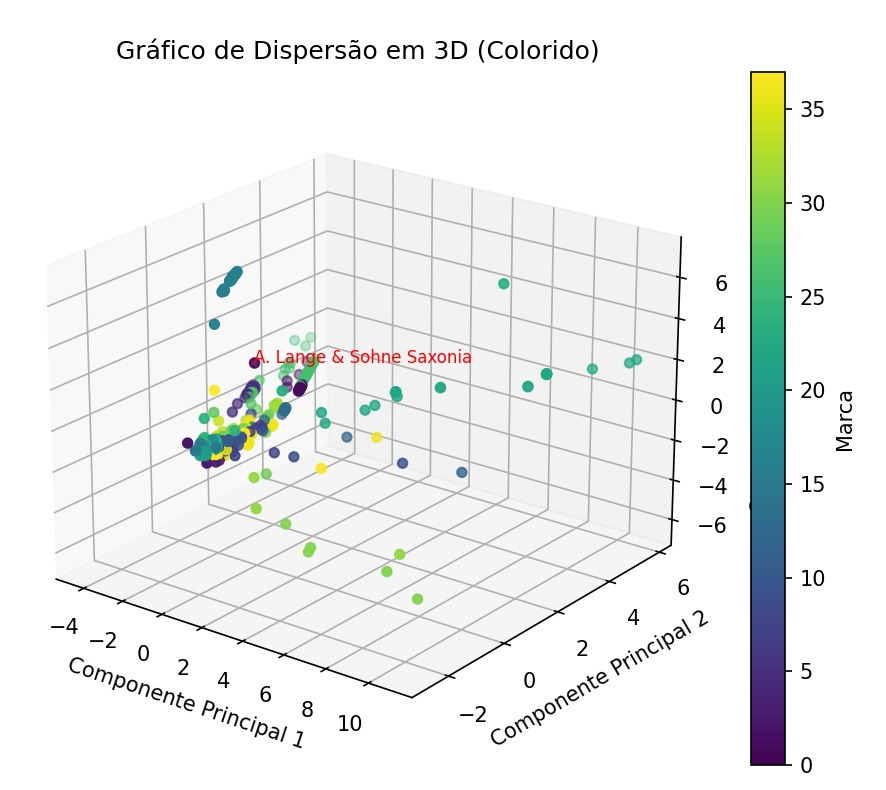
\includegraphics[width=14cm]{figura4.jpg}
\end{center}
\textbf{A.Lange & Sohne - Saxonia é  dado com autovalor mais significativo, sua posição está indicada no gráfico}
\begin{center}
    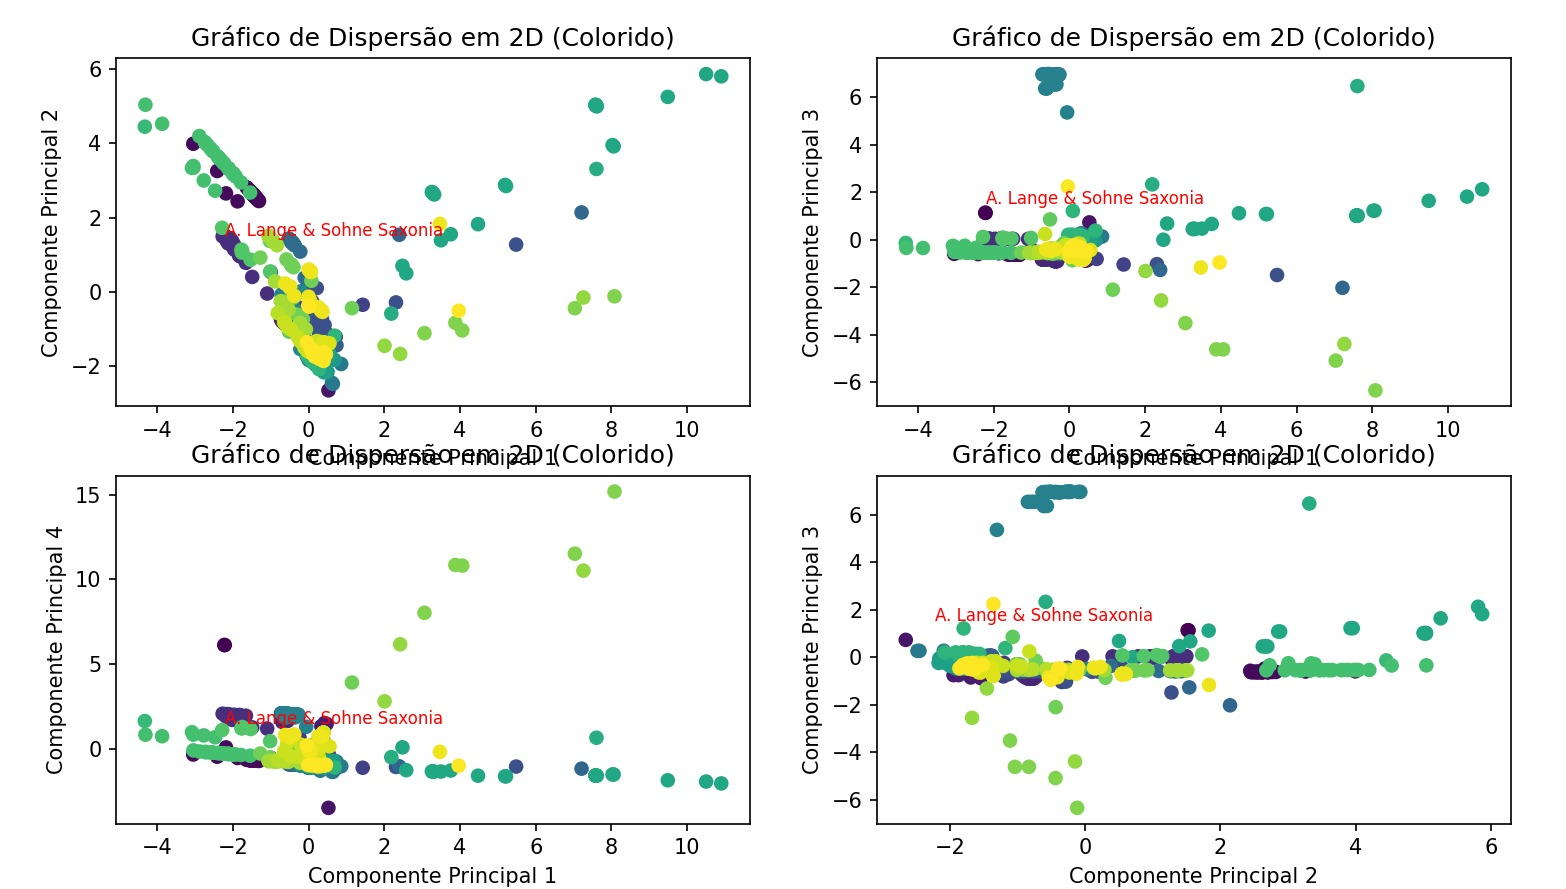
\includegraphics[width=14cm]{figura5.jpg}
    \textbf{Exemplo de 4 gráficos de dispersão em busca do melhor padrão.}
\end{center}


\subsection{Conclusão}
Concluímos que a análise de PCA realizada pelo código fornece insights sobre a estrutura dos dados de relógios de luxo, destacando as principais variáveis que influenciam a variação nos dados e possibilitando a visualização e interpretação dos padrões encontrados.


\end{document}